\chapter{Estado del arte}

En este capítulo se va a hacer una introducción teórica a los pilares en los que se asienta este trabajo, SHM e IA, y sus aplicaciones en la industria aeroespacial.. 

\section{Structural Health Monitoring}

Structural Helath Monitoring (SHM) es el proceso de identificar daños en estructuras de forma no destructiva mediante el uso de sensores integrados \cite{SHM_Aero_3}. Por lo tanto, es necesario tener el concepto de daño bien definido. Se puede definir un daño como los cambios en el material y/o en las propiedades geométricas de un sistema estructural, incluyendo cambios en las condiciones de contorno y conectividad del mismo, que pueden afectar de manera adversa al funcionamiento presente y futuro del sistema \cite{dam}. 

La gran ventaja de este proceso frente a las NDI de los que evoluciona es que se puede aplicar en tiempo real, incluyendo durante la operación del vehículo. Con esto se consigue, no solo tener un conocimiento total de la salud estructural, sino que también se puede llegar a monitorizar la magnitud de las cargas a las que las estructuras instrumentadas están sometidas.


El SHM se realiza en cuatro pasos principales:\\

\begin{enumerate}
    \item \textbf{Evacuación operacional}: para aplicar la técnica de SHM, la evaluación operativa es el paso fundamental. Estudia los problemas y sus consecuencias que conducen a monitorizar las estructuras. La evaluación estructural trata de buscar solución a varias preguntas, tales como:
    \begin{itemize}
        \item[\tiny{\textbullet}] ¿qué tipo de daño se busca en la estructura monitorizada?
        \item[\tiny{\textbullet}] ¿a qué condiciones ambientales y operativas está sometido la estructura monitorizada mientras se lleva a cabo el proceso de SHM?
        \item[\tiny{\textbullet}] ¿Cuáles son las restricciones de la transferencia de datos a través del sistema SHM a causa de la operación del vehículo?
        \item[\tiny{\textbullet}] ¿cuáles son las ventajas del SHM en la vida segura del vehículo?
    \end{itemize}
    
    \item \textbf{Adquisición de datos}: el proceso de adquisición de datos es una parte crucial en SHM y se realiza a través de sensores integrados en la estructura. El tipo de sensores que se utilizarán está ligado a la técnica de SHM usada. En esta fase se estudia el número de sensores usados, su distribución en la estructura y  el hardware que almacenará esta información. 
    
    \item \textbf{Procesado de señales y extracción de características debidas al daño}: la parte más crítica del SHM es extraer las inferencias a partir de las señales recogidas por los sensores. Este proceso se basa en descubrir qué propiedades y áreas son afectadas por el daño junto con como varían a medida que el daño evoluciona.
    
    \item \textbf{Modelado estadístico para evaluación de las características}: el desarrollo de un modelo estadístico es el paso final del SHM. Este proceso incluye dos categorías:
    \begin{itemize}
        \item Cuando los datos recopilados pertenecen tanto a partes dañadas como a no dañadas, el modelado estadístico hace una clasificación general también conocida como aprendizaje supervisado, como puede ser el análisis de regresión y clasificación grupal.
        \item Cuando los datos proceden únicamente de estructuras dañadas, se habla de aprendizaje no supervisado.
    \end{itemize}
\end{enumerate} \vspace*{10pt}

Desde un punto de vista matemático, los sistemas SHM se puede considerar como sistemas de control realimentado, diferenciándose de éstos en los tiempos característicos y el modo de actuación sobre la planta.  %\cite{shon}

Las escalas temporales dependen de lo que el sistema busca controlar. En el caso de una grieta, los tiempos característicos son del orden de la vida operativa de la planta, en cambio, si se quiere un sistema de localización y detección de impactos, el tiempo característico se reduce a decenas de ms. 

También cambian las características espaciales, dependiendo fundamentalmente de la criticidad del daño. La longitud característica será grande cuando la tolerancia al daño permita tamaños considerables, sin embargo, en las zonas donde ésta tolerancia sera pequeña, la longitud característica también lo tendrá que ser \cite{Jaime_Tesis}.

Para funcionar, un sistema SHM medirá todas las entradas y salidas que afectan a la planta monitorizada, entendiéndose como planta aquella cuya función sea soportar o transmitir cargas, siendo fija o móvil. Los parámetros de observación serían los parámetros característicos de operación propios y los relativos al entorno. La situación anómala será aquella que comprometa el funcionamiento presente y futuro de la planta, en su conjunto, dentro de las condiciones de diseño \cite{civil}.\\

Así pues, tenemos que el SHM es en esencia un sistema autónomo para inspeccionar y detectar daños en estructuras con una mínima intervención humana. En la Figura \ref{sistema} se puede ver representada esta idea \cite{Jaime_Tesis}.

\vspace*{10pt}
\begin{figure}[ht]
    \centering
    \tikzstyle{block} = [rectangle, draw=black, thick, text centered, rounded corners]
    \tikzstyle{empty} = [rectangle, thick, text width=7em, text centered, rounded corners,minimum height=5mm, minimum width=5mm]
    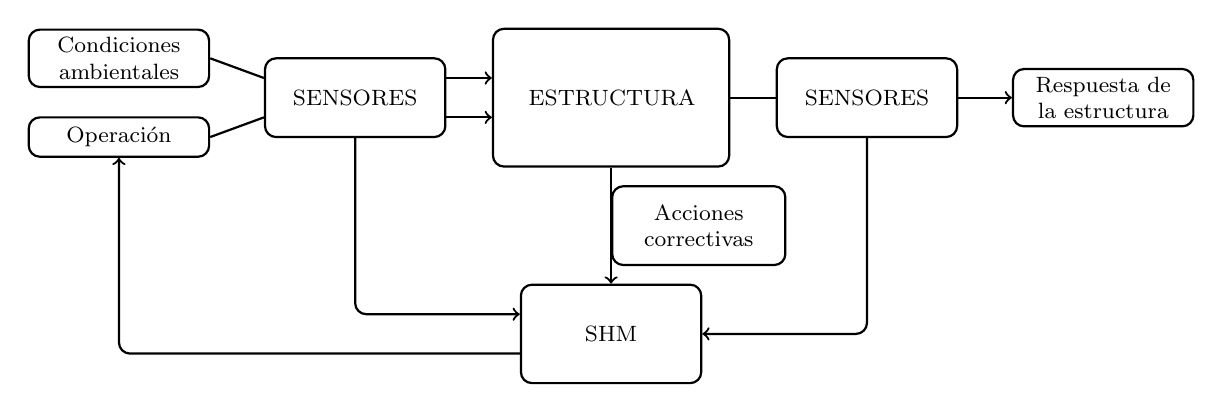
\begin{tikzpicture}[thick]
        \shorthandoff{<>}
        \footnotesize
        \node[block]  (estructura)  [minimum height=17.5mm, minimum width=30mm] {ESTRUCTURA};
        \node[block,yshift=-20mm]  (shm)  [below of=estructura,minimum width=22.5mm, minimum height=12.5mm] {SHM};
        \node[block,xshift=-22.5mm]   (sensores1)     [left of=estructura, minimum width=20mm, minimum height=10mm]  {SENSORES};
        \node[empty,xshift=-20mm,yshift=5mm]   (conam)     [left of=sensores1]  {Condiciones ambientales};
        \node[empty,xshift=-20mm,yshift=-5mm]   (op)     [left of=sensores1]  {Operación};
        \node[block,xshift=22.5mm]    (sensores2)     [right of=estructura, minimum width=20mm, minimum height=10mm]  {SENSORES}; 
        \node[empty,xshift=20mm]   (res)     [right of=sensores2]  {Respuesta de la estructura};
        
        \draw[->] (estructura.south)  -- (shm.north) node [right,text width=2cm,text centered,midway]{Acciones correctivas};
        \draw[-] (conam.east) -- ([yshift=2.5mm]sensores1.west);
        \draw[-] (op.east) -- ([yshift=-2.5mm]sensores1.west);
        \draw[->] ([yshift=2.5mm]sensores1.east) -- ([yshift=2.5mm]estructura.west);
        \draw[->] ([yshift=-2.5mm]sensores1.east) -- ([yshift=-2.5mm]estructura.west);
        \draw[-] (estructura.east) -- (sensores2.west);
        \draw[->] (sensores2.east) -- (res.west);
        \draw[->,rounded corners] (sensores1.south) |- ([yshift=2.5mm]shm.west);
        \draw[->,rounded corners] ([yshift=-2.5mm]shm.west) -|  (op.south);
        \draw[->,rounded corners] (sensores2.south) |- (shm.east);
    \end{tikzpicture}
    \caption{SHM como sistema realimentado}
    \label{sistema}
\end{figure}
\vspace*{10pt}

%----------------------------------------------------------------------%

\section{Monitorización de estructuras aeronáuticas - SHM 5 pags (SHM a día de hoy – futuros desarrollos)}

Dentro de la gran variedad de estructuras en las que se puede aplicar el SHM, este trabajo se va a centrar en estructuras aeronáuticas fabricadas con material compuesto. Como ya se ha introducido en el primer paso del SHM, \textit{Evaluación operacional}, hay una serie de preguntas que se necesitan responder para elegir el sistema óptimo para monitorizar una estructura determinada dentro de todas las que componen una aeronave. 

Será necesario dar respuesta a las siguientes cuestiones:
\begin{enumerate}
    \item ¿Qué estructura se quiere monitorizar?
    \item ¿Qué tipo de daño afecta a la integridad de dicha estructura?
    \item ¿Cuál va a ser la característica sensitiva al daño, o Damage Sensitive Feature (DSF), la que se 	va a usar? El DSF tendrá que ser alguna característica o parámetro medible de la estructura que sea 		modificado por la presencia del daño.
    \item ¿De qué modo el daño influye en la DSF?
\end{enumerate}

Una vez que todas estas preguntas tengan respuesta, se tendrá toda la información necesaria para elegir una estrategia global de SHM apropiada para el objetivo que se ha fijado. A continuación, se van a responder estas cuestiones para el caso de estructuras aeronáuticas.\\

\subsection{Estructuras aeronáuticas}

No todas las estructuras que componen una aeronave están sometidas al mismo tipo de cargas y, por lo tanto, no presentan los mismos problemas ni se usan los mismos criterios de diseño para toda la aeronave.

\begin{figure}[ht]
    \centering
    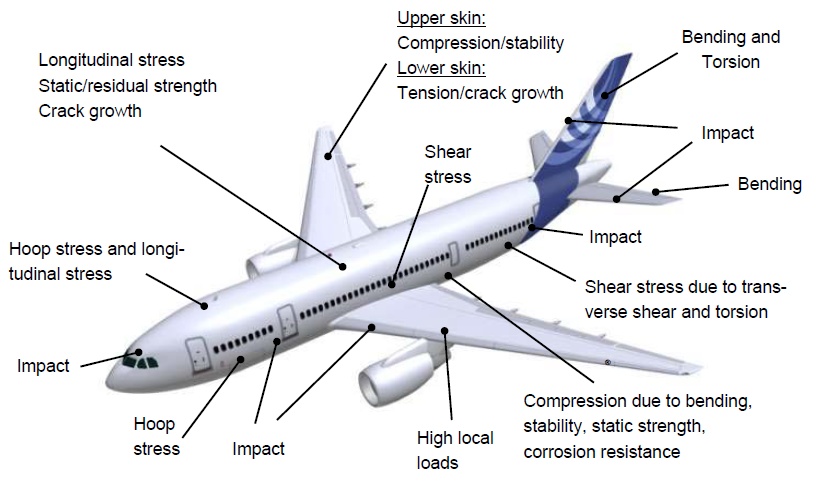
\includegraphics[width=125mm]{2/Fotos/Aircraft_Sress.png}
    \caption{Problemas asociados a las estructuras de una aeronave} % \cite{stress}
    \label{stress}
\end{figure}

En aeronáutica, la inmensa mayoría de partes se diseñan a fatiga. Esto quiere decir que, para un número determinado de ciclos y con un espectro determinado de cargas, la pieza o estructura no compromete la integridad global de la aeronave.

Dentro del diseño a fatiga hay otras dos tendencias, el diseño a vida segura o a tolerancia al daño. En las estructuras diseñadas bajo el criterio de vida segura granizan que, mientras no se supere el espectro de carga, la integridad estructural no peligra. En cambio, el diseño de tolerancia al daño tiene en cuenta que en el propio proceso de fabricación se generan grietas en el material y asume que estas grietas van a crecer, por lo que toma medidas para asegurar que no se produzcan fallos catastróficos \cite{criterios}. 

\vspace*{10pt}
\begin{figure}[ht]
    \centering
    \begin{tikzpicture}[edge from parent fork down]
        \tikzstyle{every node}=[rectangle, draw=black, thick, text width=7em, text centered, rounded corners,minimum height=5mm, minimum width=20mm,minimum height=10mm]
        \tikzstyle{edge from parent}=[black,-,thick,draw]
        \footnotesize
        \node {Diseño a Fatiga}
        child {node [xshift=-7.5mm] {Vida segura}}
        child {node [xshift=7.5mm] {Tolerancia al daño}
        child {node [xshift=-7.5mm] {Fallo seguro}
        child {node [xshift=-7.5mm] {Bloqueo de grieta}}
        child {node [xshift=7.5mm] {Camino de carga múltiple}}}
        child {node [xshift=7.5mm] {Crecimiento lento}}
        };
    \end{tikzpicture}
    \caption{Criterios de diseño \cite{criterios}}
    \label{des_cri}
\end{figure}
\vspace*{10pt}

Usando las Figuras \ref{stress} y \ref{des_cri} se puede tener una idea general de la estructura bajo estudio y responder a la primera pregunta. El siguiente paso será diferenciar entre los distintos daños que pueden sufrir estas estructuras.

%------------%

\subsection{Daños en estructuras aeronáuticas}

% En una estructura aeronáutica, se puede definir un daño como los cambios en el material y/o en las propiedades geométricas de un sistema estructural, incluyendo cambios en las condiciones de contorno y conectividad del mismo, que pueden afectar de manera adversa al funcionamiento presente y futuro del sistema \cite{dam}.\\

% Como este trabajo se va a centrar en daños sobre estructuras fabricadas en material compuesto, 
 
% De forma general, se pueden organizar los daños que sufren las estructuras aeronáuticas dentro de las siguientes categorías \cite{Jaime_Tesis}:

% \begin{itemize}
%     \item[\textbullet] \textbf{Daño accidental}: daño fortuiro y no predecible que se produce en la estructura. Por ejemplo, un impacto de pájaro.
%     \item[\textbullet] \textbf{Daño por fatiga}: este es un tipo de daño predecible, derivado de la acción de las cargas cíclicas en la misma. Un ejemplo son las grietas que aparecen en el perímetro de agujeros.
%     \item[\textbullet] \textbf{Daño ambiental}: este tipo no es predecible, se produce en la estructura por acción del medio ambiente en el que opera la estructura. Uno de los ejemplos es la corrosión.
%     \item[\textbullet] \textbf{Daño operacional}: al igual que los accidentales, es un daño no predecible y fortuito que se produce en la estructura derivado de la operación de la misma. Un caso común es una sobrecarga en la maniobra de aterrizaje.
% \end{itemize}

% Como ya se ha comentado anteriormente, este trabajo se va a centrar en estructuras fabricadas en Material Compuesto. Los modos de fallo que se producen en este tipo de material son diferentes a los que ocurren en las estructuras metálicas \cite{dam_comp} y a continuación se presenta un breve resumen de estos tipos característicos de daños \cite{comp}.

% \begin{itemize}
%     \item[\textbullet] \textbf{Daño por tracción}: este fallo es producido por varios mecanismos de daño que ocurren secuencialmente. Usando como referencia la Figura \ref{traccion} se tiene un laminado [0,90,0] con una carga longitudinal aplicada en la orientación 0º. Cuando comienza un ciclo de carga, primero se rompe la lámina orientada a 90º ya que la resina es la que soporta los mayores esfuerzos. Cuando aumenta la carga, comienzan a aparecer delaminaciones entre las pieles debido a tensiones generadas por efectos tridimensionales. Si sigue aumentando la carga, se llega a rotura final de la fibra.
%     \begin{figure}[ht]
%         \centering
%         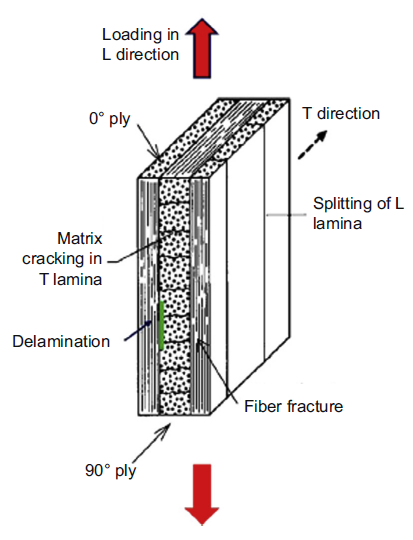
\includegraphics[width=50mm]{2/Fotos/traccion.png}%
%         \caption{Tracción axial}
%         \label{traccion}
%     \end{figure}
    
%     \item[\textbullet] \textbf{Daño en compresión}: cuando se somete a estructura a compresión axial, el compuesto falla por pandeo. En una escala local, el material falla por el mecanismo de micropandeo. Al estar las fibras en una matriz flexible, al aplicar la carga las fibras se empiezan a ondular, como se ve en la Figura \ref{pandeo-a}. Conforme aumenta la carga la ondulación aumenta hasta que se produce el fallo en forma de \textit{kink bands}, en las Figuras \ref{pandeo-b} y \ref{pandeo-c} se puede apreciar el fenómeno.
%     \begin{figure}[ht]
%         \centering
%         \subfloat[Ondulación de las fibras]{%
%           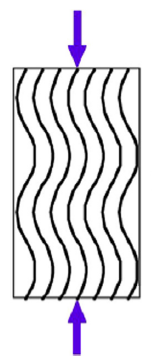
\includegraphics[width=22.5mm]{2/Fotos/pandeo-a.png}%
%           \label{pandeo-a}%
%         }\qquad
%         \subfloat[Falla local de banda]{%
%           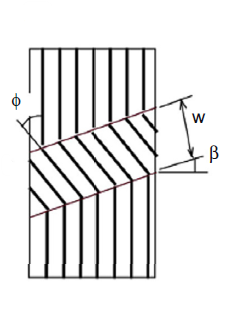
\includegraphics[width=35mm]{2/Fotos/pandeo-b.png}%
%           \label{pandeo-b}%
%         }
%         \subfloat[Micrografía de falla local de banda]{%
%           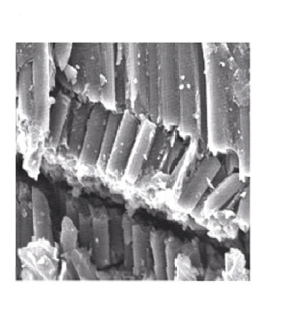
\includegraphics[width=45mm]{2/Fotos/pandeo-c.png}%
%           \label{pandeo-c}%
%         }
%         \caption{Daño por compresión en compuestos por micropandeo}
%     \end{figure}
    
%     \item[\textbullet] \textbf{Daños en agujeros de unión}: cuando se quiere unir una pieza metálica con otra de compuesto, un método ampliamente usado es la unión con elementos mecánicos, lo que lleva a realizar agujeros y tiene una gran penalización en la rigidez y fatiga. Se pueden dar causados por tracción, Figura \ref{agujero-a}, o por compresión, Figura \ref{agujero-b}.
%     \begin{figure}[ht]
%         \centering
%         \subfloat[Fallos por tracción]{%
%           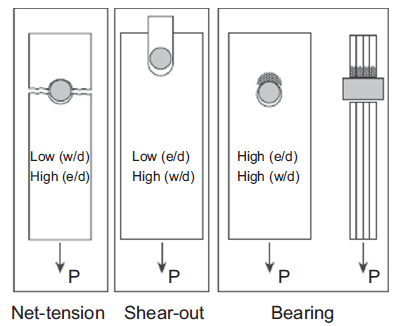
\includegraphics[width=65mm]{2/Fotos/agujero-a.png}%
%           \label{agujero-a}%
%         }\qquad
%         \subfloat[Fallos por compresión]{%
%           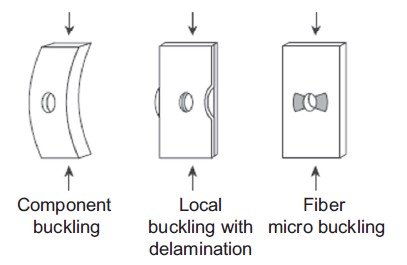
\includegraphics[width=75mm]{2/Fotos/agujero-b.png}%
%           \label{agujero-b}%
%         }
%         \caption{Distintos daños en agujeros de unión}
%     \end{figure}
    
%     \item[\textbullet] \textbf{Daño por impacto}: este tipo de daño no es importante en estructuras metálicas, sin embargo, un impacto de baja velocidad puede generar daños importantes y sin dejar ninguna marca en la superficie. Cuando el impacto es de baja energía puede generar delaminaciones y si tiene la energía suficiente producirá desconchado en la superficie opuesta al impacto. Se puede ver el esquema de las etapas que sufre un laminado unidireccional bajo una carga cíclica en la Figura \ref{delaminacion}. 
%     \begin{figure}[ht]
%         \centering
%         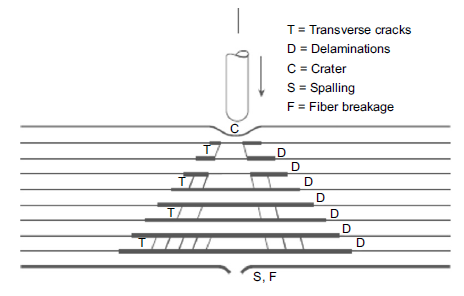
\includegraphics[width=125mm]{2/Fotos/delamination.png}%
%         \caption{Consecuencias de un impacto en material compuesto}
%         \label{delaminacion}
%     \end{figure}
    
%     \item[\textbullet] \textbf{Daño por fatiga}: la fatiga en compuestos es más complicada que en materiales metálicos. En la Figura \ref{fatiga}. La evolución del daño por estas fases depende del nivel de carga en el ciclo de fatiga.
%     \begin{figure}[ht]
%         \centering
%         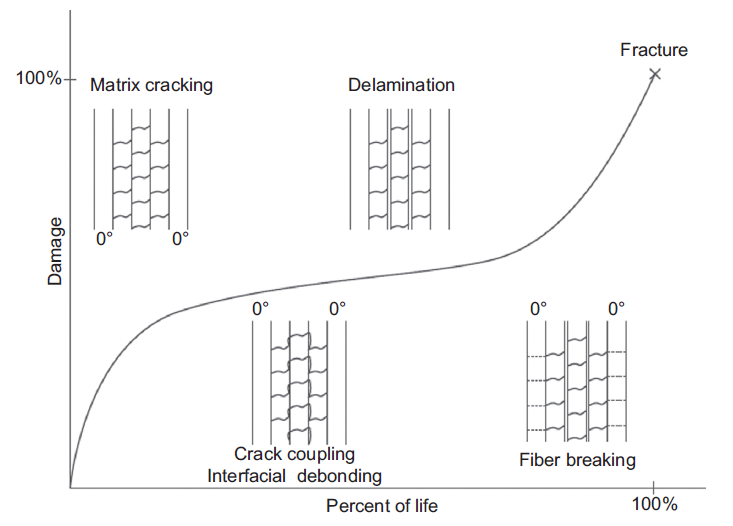
\includegraphics[width=125mm]{2/Fotos/fatiga.png}%
%         \caption{Etapas de crecimiento de daño en fatiga}
%         \label{fatiga}
%     \end{figure}
    
%     \item[\textbullet] \textbf{Daño en estructuras sandwich}: los paneles sandwich de polímero reforzado con fibra de carbono (CFRP)son mucho más sucreptibles al daño por impacto que los fabricados con polímero reforzado con fibra de vidrio (GFRP), y el tipo de daño predominante en cada uno de ellos es diferente. La rotura de fibra en CFRP sandwich y el aplastamiento del núcleo en los paneles fabricados con GFRP. En la Figura \ref{sandwich} se pueden ver diversos daños que estos paneles pueden sufrir.
%     \begin{figure}[ht]
%         \centering
%         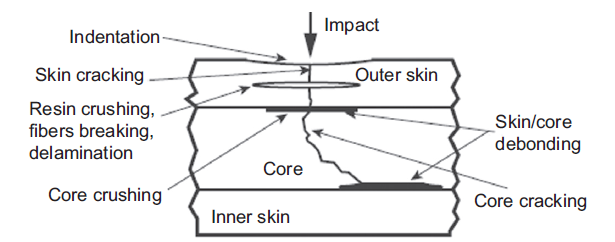
\includegraphics[width=125mm]{2/Fotos/sanwich.png}%
%         \caption{Daños típicos en paneles sandwich}
%         \label{sandwich}
%     \end{figure}
    
%     \item[\textbullet] \textbf{Daño en uniones adhesivas}: la unión adhesiva es ventajosa frente la mecánica, ya que el hacer agujeros presenta muchos problemas. Sin embargo, la fiabilidad de las uniones adhesivas no siempre se puede garantizar. La delaminación en uniones adhesivas de compuestos es el daño más frecuente, lo que reduce la rigidez de la estructura y con ello la capacidad de carga de la estructura.
% \end{itemize}

% Estos daños se pueden producir de forma conjunta y, de hecho, la inmensa mayoría de ellos aparecen en fuselajes o elementos de pared delgada.\\

% Una vez que se tiene la lista de posibles daños que pueden afectar a una estructura se necesita encontrar cuál de todos los parámetros medibles en esta estructura se ve afectado por la presencia del daño, la DSF.

% A su vez, hay que tener en cuenta como el daño modifica la DSF a medida que crece. Esta relación se llama Firma de Daño (FdD). Dicha firma puede ser algún valor relacionado con la medida o señal que se obtiene de la DSF.

% Una vez definidas la DSF y la FdD apropiadas para la estructura que se esté estudiando, se puede pasar a la elección de la tecnología SHM a aplicar.\\

% \textbf{METER LA TABLA DE JAIME CON LAS CARACTERÍSTICAS SENSITIVAS QUE SE VEN AFECTADAS POR CADA DAÑO?}


% \subsection{Tecnologías SHM}

% Una de las formas de clasificar las diferentes técnicas de SHM consiste en evaluar la física que hay detrás de ellas. Para un mejor entendimiento se ha dibujado un mapa conceptual que relaciona las tecnologías con los sensores.

% \vspace*{10pt}
% \begin{figure}[ht]
%     \centering
%     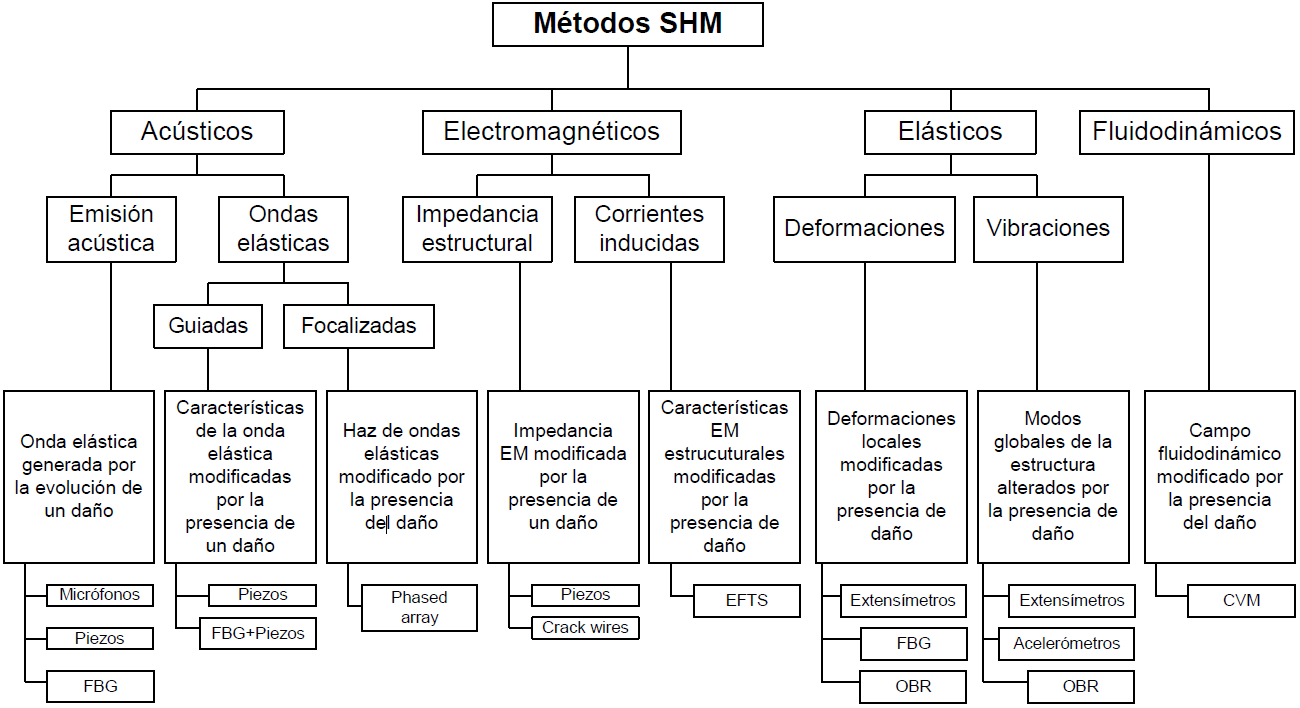
\includegraphics[width=\textwidth]{2/Fotos/shm_tec.png}
%     \caption{Tecnología SHM \cite{shm_tec}}
%     \label{}
% \end{figure}
% \vspace*{10pt}

% Una vez sabiendo los sensores y tecnologías SHM disponibles junto a los daños típicos, se puede construir una tabla para hacer más sencilla la elección de una tecnología para un determinado daño y DSF \cite{Jaime_Tesis}.

% \begin{table}[H]
%     \centering
%     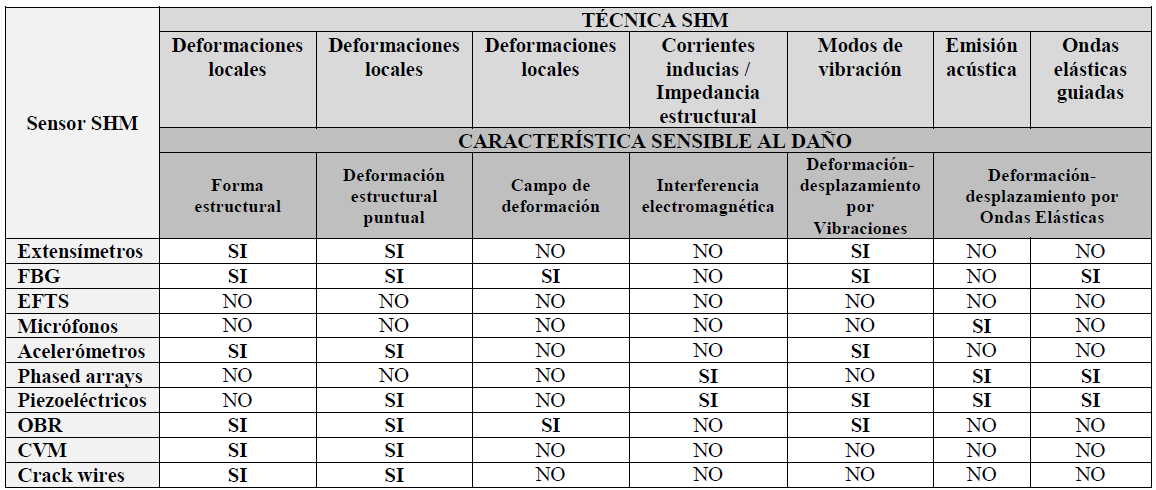
\includegraphics[width=\textwidth]{2/Fotos/DSF_tec.png}
%     \caption{Relación entre sensores y técnicas de SHM con DSF \cite{Jaime_Tesis}}
%     \label{dsf_tec}
% \end{table}



\clearpage

% -- -- %


\section{Inteligencia Artificial aplicada a SHM}  %{Machine Learning SHM}

2-3 pags

\begin{enumerate}
    \item Explicar que es la inteligencia artificial y lo tipos que hay
    \item Diferencias que hay entre Machine learning y Deep learning y por qué decidimos que el Deep Learning es mejor para nuestro objetivo
    \item Comentar las distintas redes neuronales dentro de DL y argumentos para elegir las Recurrent Neural Networks - RNN
    \item Ejemplos de IA aplicada en SHM
\end{enumerate}

\subsection{Representación gráfica del funcionamiento de una Red Neuronal}
\label{sec:funcionamiento_DL}

Aunque el campo del DL lleva unos años en auge, para la mayoría de usuarios sigue siendo una simple herramienta, es desconocido cómo funciona y mucho menos se tiene una representación gráfica de qué hace y cómo llega a los resultados.

Dado que este trabajo se va a centrar en tecnología de DL, es conveniente hacer una breve explicación de cómo una NN es capaz de clasificar diferentes grupos de datos. Para ello, esta explicación se ha basado en el gran trabajo realizado por el equipo de \textit{TensorFlow - playground} \cite{TensorFlow_playground}. Un entorno perfecto para la visualización del comportamiento de los diferentes parámetros que componen una Red Neuronal.\\

Lo primero de todo es saber la forma de los argumentos de entrada que, como para casi todo algoritmo, sus \textit{inputs} son números. Dependiendo del problema que se busque resolver estos datos tendrán una forma u otra, más complejos o más simples, pero en esta introducción se va a utilizar un dataset de 2 dimensiones ($x_1,x_2$) y dos clases diferentes (azul y naranja).

Los datos que se van a intentar clasificar están representados en la Figura \ref{datos}

\begin{figure}[h!]
    \centering
    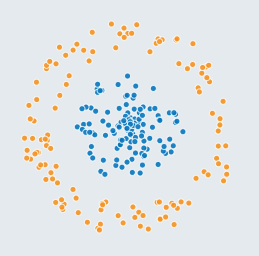
\includegraphics[width=60mm, angle=0]{2/Fotos/datos.png}
    \captionsetup{justification=centering,margin=1.25cm}
    \caption{Representación de las dos clases diferentes en dos colores}
    \label{datos}
\end{figure}

Una vez se conocen los dos grupos que se busca clasificar se va a comenzar la descripción de los elementos que componen una NN y como interactúan entre ellos. Estos elementos son:

\begin{itemize}
    \item[\tiny{\textbullet}] \textbf{Neurona}
    
    Es la unidad básica de procesamiento que compone una Red Neuronal. Estas neuronas tienen conexiones a través de las que reciben los valores de entrada y realizan una suma ponderada con ellos. Cada una de las entradas es multiplicada por un valor, llamado peso, que definirá a cual de los valores de entrada se le da más importancia. A este cálculo se le añadirá un sesgo o \textit{bias}, dicho de otro modo, se le sumará un escalar.
    
    Si se observa detenidamente la Figura \ref{perceptron} (primera neurona llamada \textit{perceptron}) se puede ver que, matemáticamente, una neurona es equivalente a una regresión lineal ($w_1 \cdot x_1 + w_2 \cdot x_2 + b = 0$).
    
    \begin{figure}[H]
        \centering
        \begin{tikzpicture}[
            init/.style={
              draw,
              circle,
              inner sep=2pt,
              font=\Huge,
              join = by -latex
            },
            squa/.style={
              draw,
              inner sep=2pt,
              font=\Large,
              join = by -latex
            },
            start chain=2,node distance=13mm
            ]
            \node[on chain=2] 
              (x2) {$x_2$};
            \node[on chain=2,join=by o-latex] 
              {$w_2$};
            \node[on chain=2,init] (sigma) 
              {$\displaystyle\Sigma$};
            % \node[on chain=2,squa,label=above:{\parbox{2cm}{\centering Activate \\ function}}]   
            %   {$f$};
            \node[on chain=2,label=above:Output,join=by -latex] 
              {$y$};
            \begin{scope}[start chain=1]
            \node[on chain=1] at (0,1.5cm) 
              (x1) {$x_1$};
            \node[on chain=1,join=by o-latex] 
              (w1) {$w_1$};
            \end{scope}
            \begin{scope}[start chain=3]
            \node[on chain=3] at (0,-1.5cm) 
              (x3) {$x_3$};
            \node[on chain=3,label=below:Weights,join=by o-latex] 
              (w3) {$w_3$};
            \end{scope}
            \node[label=above:\parbox{2cm}{\centering Bias \\ $b$}] at (sigma|-w1) (b) {};
            
            \draw[-latex] (w1) -- (sigma);
            \draw[-latex] (w3) -- (sigma);
            \draw[o-latex] (b) -- (sigma);
            
            \draw[decorate,decoration={brace,mirror}] (x1.north west) -- node[left=10pt] {Inputs} (x3.south west);
        \end{tikzpicture}
        \captionsetup{justification=centering,margin=1.25cm}
        \caption{Representación del \textit{perceptron}}
        \label{perceptron}
    \end{figure}
    
    En una regresión lineal bidimensional, ajustando los pesos ($w_1,w_2$) se modifica la recta que separa el plano ($x_1,x_2$) en dos regiones. En el ejemplo que se está resolviendo, por muy bien que se ajusten estos pesos, con una neurona solo se puede llegar a separar el plano en dos regiones, como se ve en la Figura \ref{neurona}.
    
    \begin{figure}[h!]
        \centering
        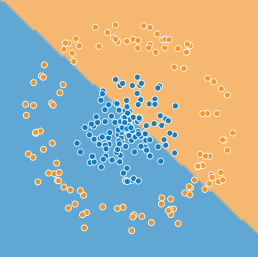
\includegraphics[width=60mm, angle=0]{2/Fotos/neurona.png}
        \captionsetup{justification=centering,margin=1.25cm}
        \caption{Clasificación de datos con una sola neurona}
        \label{neurona}
    \end{figure}
    
    Para definir que región del plano es asignada a la clase azul o naranja se utiliza la siguiente expresión:
    
    \begin{equation}
        w_1 \cdot x_1 + w_2 \cdot x_2 + b = y \hspace*{5pt}
        \begin{cases}
            y \geq 0, & naranja\\
            y < 0, & azul%\text{otherwise}
        \end{cases}
        \label{eq:percepron}
    \end{equation}

    Por lo tanto, la neurona se puede sintetizar un una función. Como una neurona no consigue separar las dos regiones de puntos de forma efectiva, hace que sea necesario dar un paso más.
    
    
    %https://tex.stackexchange.com/questions/132444/diagram-of-an-artificial-neural-network
    
    \item[\tiny{\textbullet}] \textbf{Capas}
    
    Para modelizar conocimiento complejo no es suficiente con utilizar una única neurona, es necesario concatenar varias de ellas. Una forma de colocar las neuronas sería una debajo de otra en forma de columna, lo que se define como, en la misma capa.
    
    \begin{figure}[H]
        \centering
        \tikzset{%
          every neuron/.style={
            circle,
            draw,
            minimum size=1cm
          },
          neuron missing/.style={
            draw=none, 
            scale=4,
            text height=0.333cm,
            execute at begin node=\color{black}$\vdots$
          },
        }
        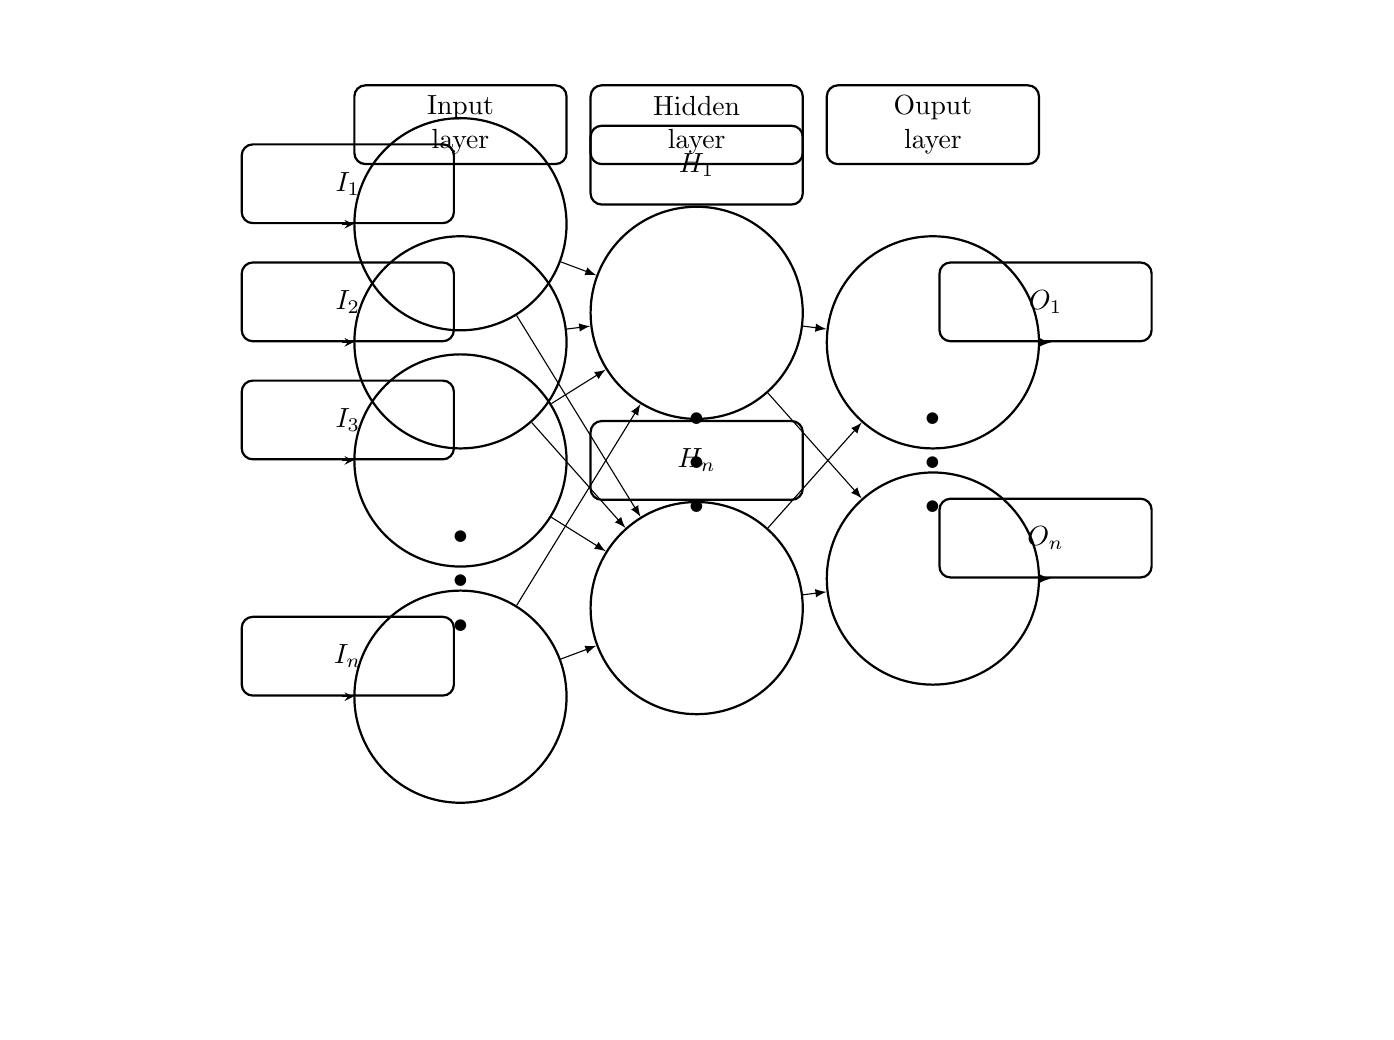
\begin{tikzpicture}[x=1.5cm, y=1.5cm, >=stealth]
            \foreach \m/\l [count=\y] in {1,2,3,missing,4}
              \node [every neuron/.try, neuron \m/.try] (input-\m) at (0,2.5-\y) {};
            \foreach \m [count=\y] in {1,missing,2}
              \node [every neuron/.try, neuron \m/.try ] (hidden-\m) at (2,2-\y*1.25) {};
            \foreach \m [count=\y] in {1,missing,2}
              \node [every neuron/.try, neuron \m/.try ] (output-\m) at (4,1.5-\y) {};
            \foreach \l [count=\i] in {1,2,3,n}
              \draw [<-] (input-\i) -- ++(-1,0)
                node [above, midway] {$I_\l$};
            \foreach \l [count=\i] in {1,n}
              \node [above] at (hidden-\i.north) {$H_\l$};
            \foreach \l [count=\i] in {1,n}
              \draw [-latex] (output-\i) -- ++(1,0)
                node [above, midway] {$O_\l$};
            \foreach \i in {1,...,4}
              \foreach \j in {1,...,2}
                \draw [-latex] (input-\i) -- (hidden-\j);
            \foreach \i in {1,...,2}
              \foreach \j in {1,...,2}
                \draw [-latex] (hidden-\i) -- (output-\j);
            \foreach \l [count=\x from 0] in {Input, Hidden, Ouput}
              \node [align=center, above] at (\x*2,2) {\l \\ layer};
        \end{tikzpicture}
        \captionsetup{justification=centering,margin=1.25cm}
        \caption{Representación de las capas de una red}
        \label{capas}
    \end{figure}
    
    Como se representa en la Figura \ref{capas}, las capas se pueden concatenar de manera secuencial, una detrás de otra y dependiendo de dónde estén colocadas tendrán un nombre u otro. La capa que recibe primero los argumentos de entrada se llama \textit{Input layer}, la que calcula el argumento de salida se llama \textit{Output layer} y todas las capas que estén entre estas dos, se llamarán \textit{Hidden layers}. 
    
    La concatenación secuencial de las capas hace que la red sea capaz de aprender conocimiento jerarquizado y es lo que da nombre al Deep Learning (Aprendizaje Profundo). Dicho de otro modo, si a la red se le introduce una imagen de un coche, es capaz de aprender que un coche no es un objeto único, una capa sintetiza lo que es una rueda, la siguiente lo que es una puerta y las últimas capas son capaces de juntar toda esa información para construir la idea de coche como un conjunto de objetos.
    
    Las neuronas dentro de la misma capa lo que permiten es diversificar el conocimiento. Cada neurona se especializa en una parte de la información ajustando los pesos para dar más importancia a un canal de entrada u otro.
    
    Juntando lo explicado anteriormente se entiende mejor este concepto de aprendizaje. Una red parte de una cantidad grande de datos, los píxeles de una imagen, por ejemplo. La capa de entrada será la que primero reciba la información, por ello necesitará muchas neuronas para procesarla y extraer de ella qué zonas de la imagen son más importantes. A medida que se va avanzando, cada una de las capas tiene que desglosar cada vez más la información sintetizada que le ha llegado de la capa anterior, por lo que necesitará menos neuronas, su nivel de abstracción de conocimiento aumenta.
    
    \begin{figure}[h!]
        \centering
        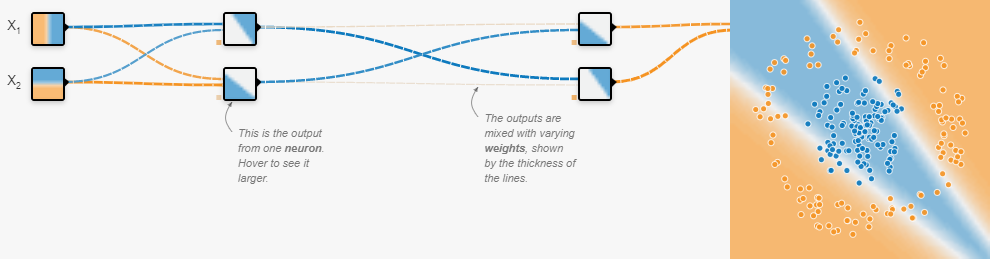
\includegraphics[width=135mm, angle=0]{2/Fotos/capas.png}
        \captionsetup{justification=centering,margin=1.25cm}
        \caption{Red con dos \textit{Hidden layers} y dos neuronas en cada capa}
        \label{aplicacion_capas}
    \end{figure}
    
    La aplicación de lo explicado anteriormente se representa en la Figura \ref{aplicacion_capas}. Se puede observar en la caja que representa cada neurona que, en esencia, todas hacen una regresión lineal y que no pueden crear una frontera circular para separar el espacio. Esto se debe a que la operación matemática de concatenación de regresiones lineales termina colapsando en una regresión lineal, no puede dibujar curvas. Para conseguirlo, es necesario añadir un elemento más. 
    

    \item[\tiny{\textbullet}] \textbf{Función de activación}
    
    La necesidad de aplicar una distorsión no lineal a la salida de las neuronas convierte en indispensables a las funciones de activación. Con ellas se podrá encadenar de forma efectiva la computación de varias neuronas.
    
    \begin{figure}[h!]
        \centering
        \begin{tikzpicture}[
            init/.style={
              draw,
              circle,
              inner sep=2pt,
              font=\Huge,
              join = by -latex
            },
            squa/.style={
              draw,
              inner sep=2pt,
              font=\Large,
              join = by -latex
            },
            start chain=2,node distance=13mm
            ]
            \node[on chain=2] 
              (x2) {$x_2$};
            \node[on chain=2,join=by o-latex] 
              {$w_2$};
            \node[on chain=2,init] (sigma) 
              {$\displaystyle\Sigma$};
            \node[on chain=2,squa,label=above:{\parbox{2cm}{\centering Activate \\ function}}]   
              (f) {$f$};
            \node[on chain=2,label=above:Output] 
              (y) {$y$};
            \begin{scope}[start chain=1]
            \node[on chain=1] at (0,1.5cm) 
              (x1) {$x_1$};
            \node[on chain=1,join=by o-latex] 
              (w1) {$w_1$};
            \end{scope}
            \begin{scope}[start chain=3]
            \node[on chain=3] at (0,-1.5cm) 
              (x3) {$x_3$};
            \node[on chain=3,label=below:Weights,join=by o-latex] 
              (w3) {$w_3$};
            \end{scope}
            \node[label=above:\parbox{2cm}{\centering Bias \\ $b$}] at (sigma|-w1) (b) {};
            
            \draw[-latex] (w1) -- (sigma);
            \draw[-latex] (w3) -- (sigma);
            \draw[o-latex] (b) -- (sigma);
            
            \draw[decorate,decoration={brace,mirror}] (x1.north west) -- node[left=10pt] {Inputs} (x3.south west);
            \draw[decorate,decoration={coil,aspect=0}] (f.east) -- (y.west);
        \end{tikzpicture}
        \captionsetup{justification=centering,margin=1.25cm}
        \caption{Efecto de la función de activación sobre el output de una neurona}
        \label{perceptron_act}
    \end{figure}
    
    En cierto modo ya se estaba usando una función de activación antes de nombrarlas. En la Ecuación \ref{eq:percepron} se había usado la función escalón para separar las dos regiones del plano, pero esta función no provoca no linealidades y no es muy efectiva cuando se requieren fronteras complejas. 
    
    \vspace*{5pt}
    \begin{figure}[h!]
        \centering
        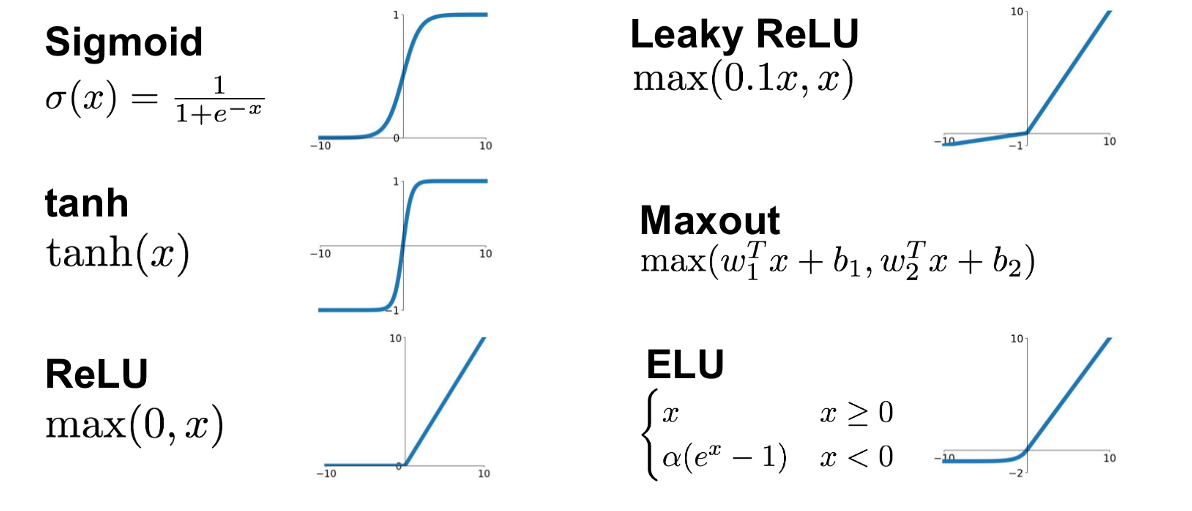
\includegraphics[width=135mm, angle=0]{2/Fotos/activation_functions.png}
        \captionsetup{justification=centering,margin=1.25cm}
        \caption{Funciones de activación más populares}
        \label{activation_functions}
    \end{figure}
    
    Las funciones de activación más conocidas están representadas en la Figura \ref{activation_functions}. Su función principal es hacer que los valores muy grandes o muy pequeños se saturen a determinado valor, dependiendo de la función elegida. 
    
    Para ver el efecto de distorsión geométrica que tienen estas funciones sobre el \textit{output} de las neuronas se usa de ejemplo la Figura \ref{single_sigmoid}. La nueva función de salida se convierte en una superficie, continua y derivable, que para cada \textit{input} ($x_1,x_2$) le corresponde una altura $y$ entre 0 y 1. 
    
    Tal y como se ha hecho anteriormente, se selecciona un valor umbral de $y$ a partir del cual se clasificarán los puntos como azules o naranjas. En la Figura \ref{single_sigmoid} este valor umbral se representa como un plano a una altura de $0.5$, por lo tanto, los puntos ($x_1,x_2$) que tras ser evaluados en la neurona saquen un valor de $y$ inferior a $0.5$ se clasificarán como \textit{naranjas} y los que den un valor superior o igual a $0.5$ se clasificarán como \textit{azules}. Esto recuerda a la Figura \ref{neurona}.

    \vspace*{5pt}
    \begin{figure}[h!]
        \centering
            \subfloat[Vista en perspectiva]{%
              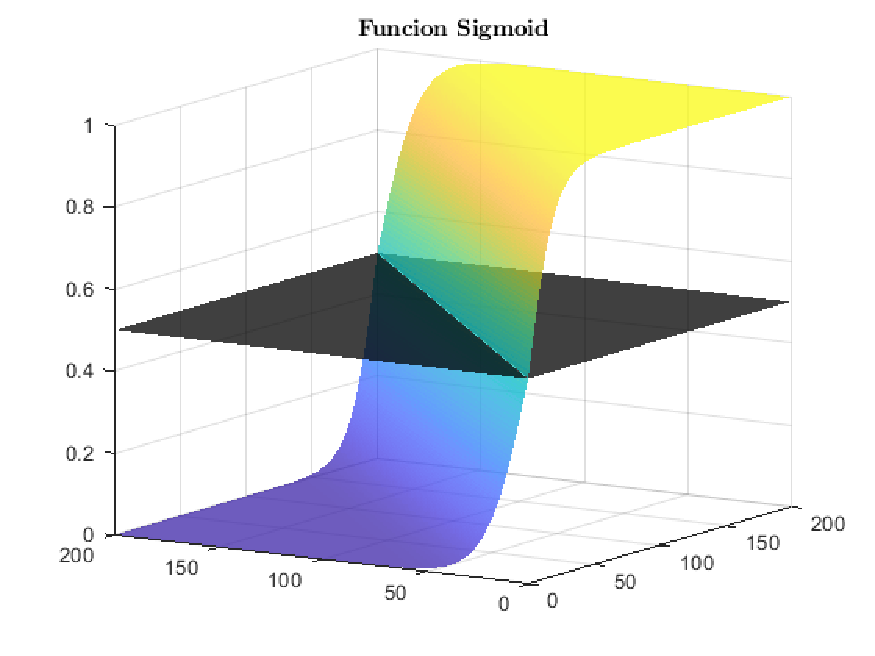
\includegraphics[width=70mm]{2/Fotos/single_sigmoid.pdf}%
              \label{}%
            }\qquad
            \subfloat[Vista perpendicular al plano de valor \textit{z = 0.5}]{%
              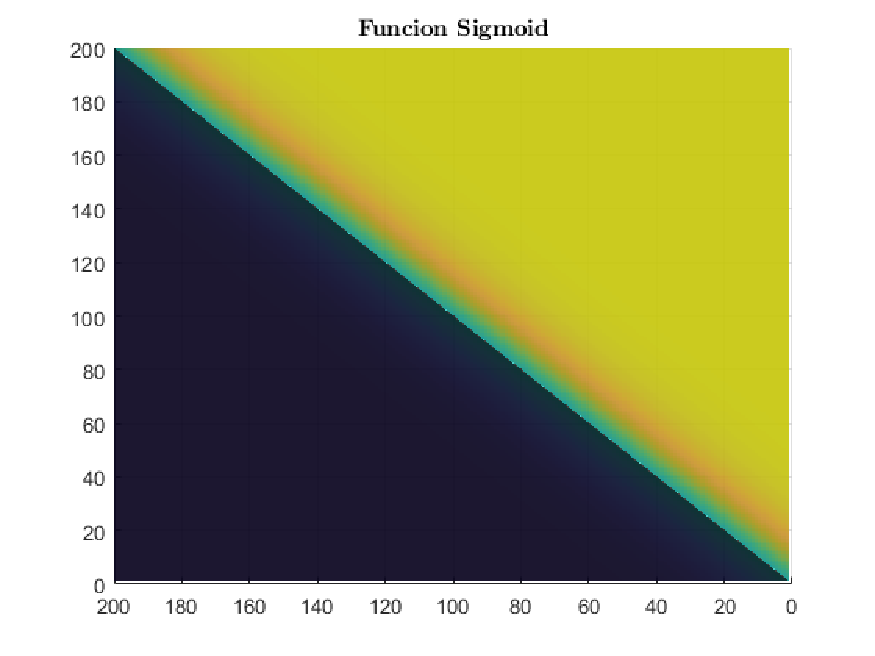
\includegraphics[width=70mm]{2/Fotos/single_sigmoid_top.pdf}%
              \label{}%
            }
        \caption{Combinación de funciones de activación}
        \label{single_sigmoid}
    \end{figure}
    
    Ahora ya se puede utilizar una \textit{hidden layer} con varias neuronas de forma efectiva. La combinación de varias neuronas hace que se sumen superficies (funciones) como la representada en la Figura \ref{single_sigmoid}, pero con diferentes orientaciones, generando superficies más complejas, Figura \ref{combinacion_sigmoid}. Igual que antes, los puntos ($x_1,x_2$) que tras ser evaluados tienen un $y$ mayor o igual a $0.5$ pertenecerán a la clase azul y los menores a la naranja.
    
    \vspace*{5pt}
    \begin{figure}[h!]
        \centering
            \subfloat[Vista en perspectiva]{%
              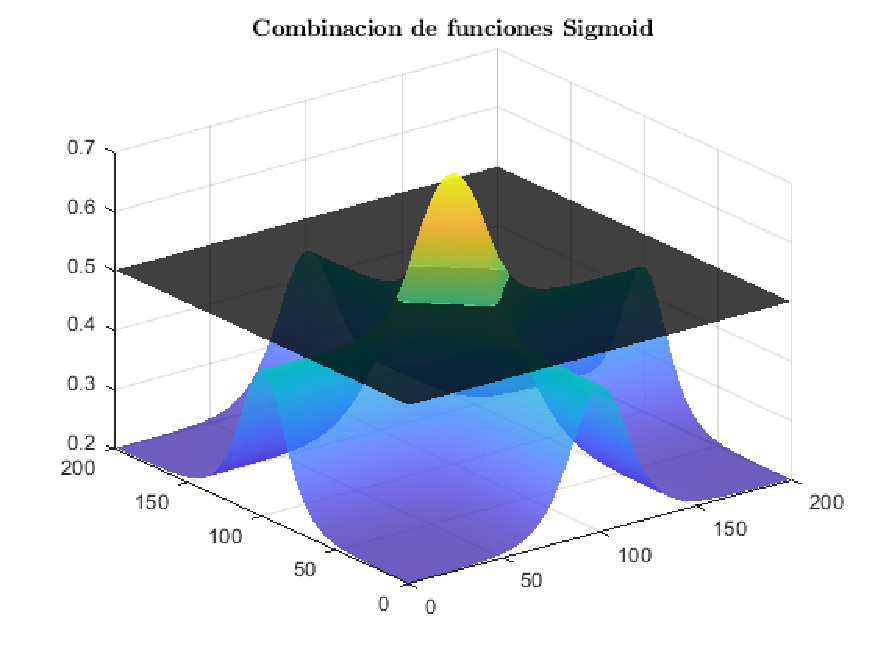
\includegraphics[width=70mm]{2/Fotos/combinacion_softmax.pdf}%
              \label{}%
            }\qquad
            \subfloat[Vista perpendicular al plano de valor \textit{z = 0.5}]{%
              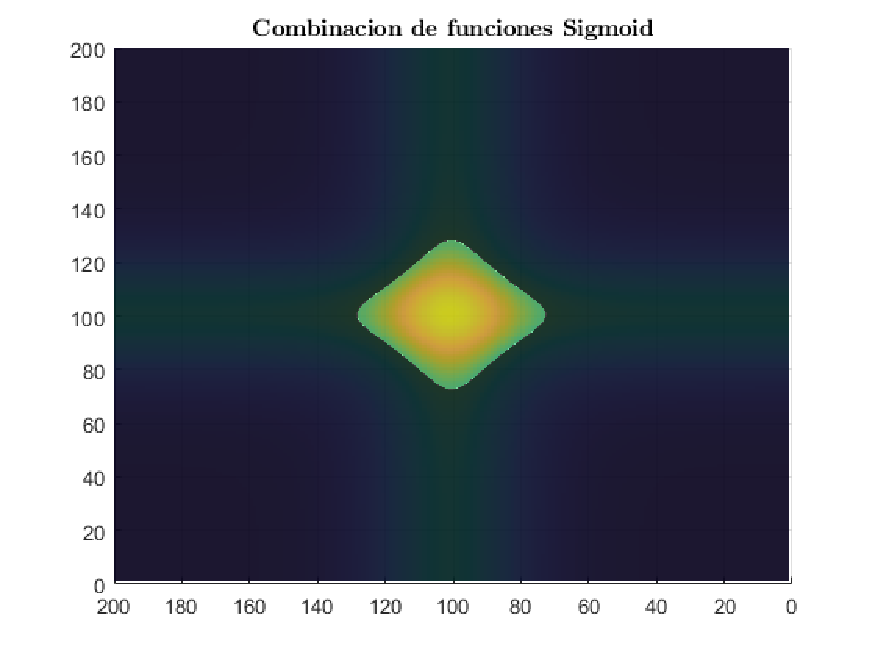
\includegraphics[width=70mm]{2/Fotos/combinacion_softmax_top.pdf}%
              \label{}%
            }
        \caption{Combinación de funciones de activación}
        \label{combinacion_sigmoid}
    \end{figure}
    
    Finalmente se puede ver en la Figura \ref{clasificacion_activacion} la aplicación de todo lo explicado. Gracias a las funciones de activación se consiguen las no linealidades necesarias para generar la superficie que separe exitosamente las dos clases de datos diferentes. 
    
    \vspace*{5pt}
    \begin{figure}[h!]
        \centering
        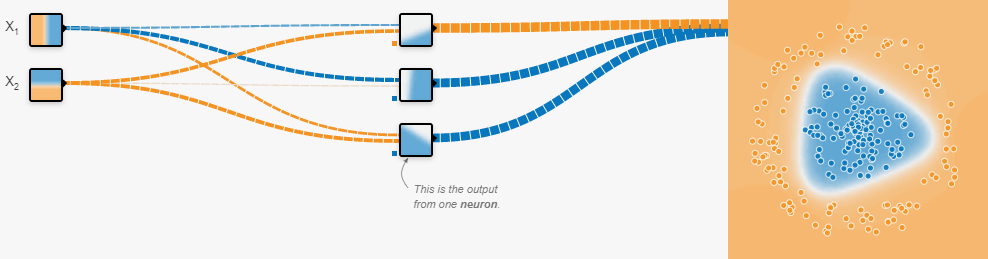
\includegraphics[width=135mm, angle=0]{2/Fotos/clasificacion_activacion.png}
        \captionsetup{justification=centering,margin=1.25cm}
        \caption{Resultado final de la clasificación}
        \label{clasificacion_activacion}
    \end{figure}
    
    Las neuronas de la Figura \ref{clasificacion_activacion} están unidas mediante unas líneas discontinuas de diferente color y grosor. Esto representa qué pesos son mayores y que zona perturban más. Los pesos son los elementos que ajustan las funciones de activación para conseguir la superficie final que mejor realice la clasificación. Pero, ¿cómo se realiza el ajuste de los pesos?
    
    \item[\tiny{\textbullet}] \textbf{Entrenamiento}
    
    Se llama entrenamiento al proceso de aprendizaje automático que utilizan las redes neuronales para ajustar sus parámetros internos. El algoritmo que hizo posible que la optimización de parámetros en DL fuera eficiente se llama \textit{backpropagation} y es el responsable del final del \textit{Invierno de la Inteligencia Artificial}
    
    Para llevar a cabo el proceso de optimización es necesario calcular las derivadas parciales de cada uno de los parámetros de la red con respecto a la función de error. Una vez se consigan las derivadas, se utilizará el algoritmo de descenso del gradiente para variar los parámetros y minimizar la función de error.
    
    La función de error ($E$) puede ser, por ejemplo, la suma de las distancias de cada punto a la frontera de su clase. Volviendo a la Figura \ref{neurona}, los puntos azules que se encuentran en la región naranja aumentarán mucho el valor de la función de error, mientras que los que están en la región azul no aumentarán casi su valor. La variación de la función de error respecto a un pequeño cambio los parámetros se representa matemáticamente como el gradiente gradiente: $\frac{\partial E}{\partial w}$.
    
    Como se ve en la Figura \ref{fig:prop_error}, el peso asociado a una de las primeras conexiones afecta a prácticamente todas las conexiones posteriores y por lo tanto, también influirán en su gradiente. Esto hace que el aprendizaje de este primer peso sea especialmente complicado y convierte en esencial la utilización del \textit{backpropagation} para el proceso de optimización.
    
    \begin{figure}[h!]
        \centering
        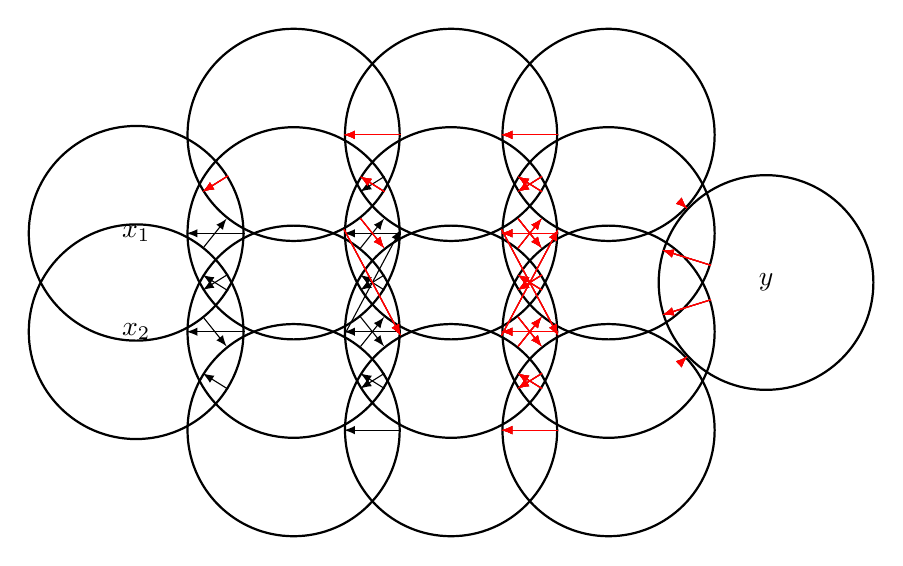
\begin{tikzpicture}
        	\tikzstyle{place}=[circle, draw=black, minimum size = 8mm]
        	% Input
        	\foreach \x in {1,...,2}
        		\draw node at (0, -1.25-\x*1.25) [place] (first_\x) {$x_\x$};
        	% Hidden 1
         	\foreach \x in {1,...,4}
         		\node at (2, -\x*1.25) [place] (second_\x){};%{$n_{1,\x}$};
        	% Hidden 2
        	\foreach \x in {1,...,4}
        		\node at (4, -\x*1.25) [place] (third_\x){};%{$n_{2,\x}$};
        	% Hidden 3
         	\foreach \x in {1,...,4}
         		\node at (6, -\x*1.25) [place] (fourth_\x){};%{$n_{3,\x}$};
        	% Output
        	\foreach \x in {1,...,1}
            		\node at (8, -\x*3.125) [place] (fifth_\x){$y$};
        	%---------------------%
        	% Input -> Hidden 1
        	\foreach \i in {1,...,2}
        		\foreach \j in {1,...,4}
        			\draw [-latex] (first_\i) to (second_\j);
        	% Hidden 1 -> Hidden 2
        	\foreach \i in {1,...,4}
        		\foreach \j in {1,...,4}
        			\draw [-latex] (second_\i) to (third_\j);
        	% Hidden 1 -> Hidden 3
        	\foreach \i in {1,...,4}
        		\foreach \j in {1,...,4}
        			\draw [-latex] (third_\i) to (fourth_\j);
        	% Hidden 3 -> Output
        	\foreach \i in {1,...,4}
    		\foreach \j in {1,...,1}
        			\draw [-latex] (fourth_\i) to (fifth_\j);
            %---------------------%
            \foreach \k in {1,...,3}{
                % Input -> Hidden 1
                \draw[red] [-latex] (first_1) to (second_1);
                % Hidden 1 -> Hidden 2
                \foreach \i in {1,...,1}
                	\foreach \j in {1,...,4}
                		\draw[red] [-latex] (second_\i) to (third_\j);
                % Hidden 2 -> Hidden 3
                \foreach \i in {1,...,4}
                	\foreach \j in {1,...,4}
                		\draw[red] [-latex] (third_\i) to (fourth_\j);
                % Hidden 3 -> Output
                	\foreach \i in {1,...,4}
            		\foreach \j in {1,...,1}
                			\draw[red] [-latex] (fourth_\i) to (fifth_\j);
            }
        \end{tikzpicture}
        \caption{Influencia de un parámetro en la red}
        \label{fig:prop_error}
    \end{figure}
    
    Cuando la red clasifica erróneamente un \textit{input} genera un valor alto de la función de error. En una NN, el error de las últimas capas depende directamente de las capas anteriores, es decir, si se detecta que una neurona no tiene influencia sobre el error, las capas posteriores a ella tampoco lo tendrán. En esto consiste el \textit{backpropagation}, en la retropropagación de errores, lo que hace muy eficiente el proceso. En la Figura \ref{fig:back_1} se puede ver el inicio del algoritmo partiendo de la última capa.
    
    \begin{figure}[h!]
        \centering
        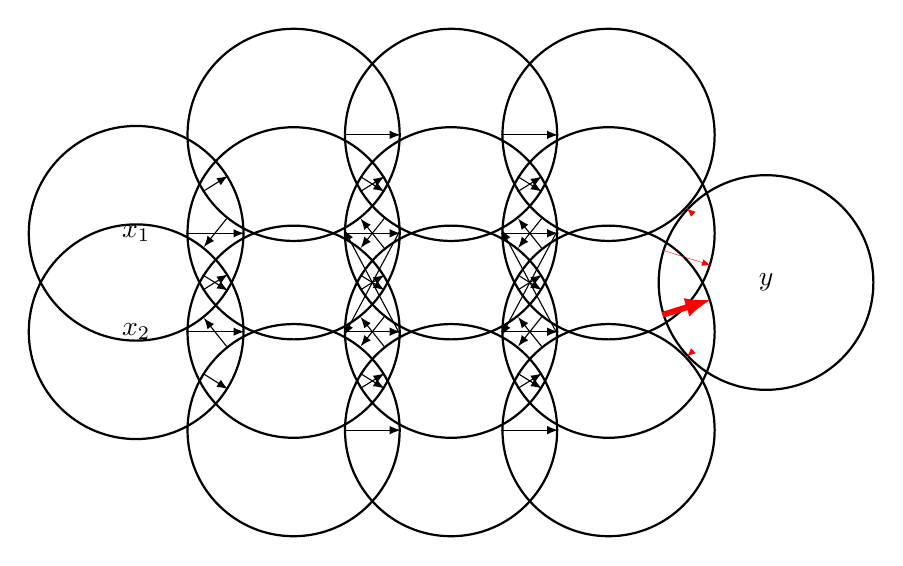
\begin{tikzpicture}
        	\tikzstyle{place}=[circle, draw=black, minimum size = 8mm]
        	% Input
        	\foreach \x in {1,...,2}
        		\draw node at (0, -1.25-\x*1.25) [place] (first_\x) {$x_\x$};
        	% Hidden 1
         	\foreach \x in {1,...,4}
         		\node at (2, -\x*1.25) [place] (second_\x){};%{$n_{1,\x}$};
        	% Hidden 2
        	\foreach \x in {1,...,4}
        		\node at (4, -\x*1.25) [place] (third_\x){};%{$n_{2,\x}$};
        	% Hidden 3
         	\foreach \x in {1,...,4}
         		\node at (6, -\x*1.25) [place] (fourth_\x){};%{$n_{3,\x}$};
        	% Output
        	\foreach \x in {1,...,1}
            		\node at (8, -\x*3.125) [place] (fifth_\x){$y$};
        	%---------------------%
        	% Input -> Hidden 1
        	\foreach \i in {1,...,2}
        		\foreach \j in {1,...,4}
        			\draw [latex-] (first_\i) to (second_\j);
        	% Hidden 1 -> Hidden 2
        	\foreach \i in {1,...,4}
        		\foreach \j in {1,...,4}
        			\draw [latex-] (second_\i) to (third_\j);
        	% Hidden 1 -> Hidden 3
        	\foreach \i in {1,...,4}
        		\foreach \j in {1,...,4}
        			\draw [latex-] (third_\i) to (fourth_\j);
        	% Hidden 3 -> Output
        	\foreach \i in {1,2,4}
    		\foreach \j in {1,...,1}
        			\draw[red, line width=0.05mm] [latex-] (fourth_\i) to (fifth_\j);
        	\draw[red, line width=0.75mm] [latex-] (fourth_3) to (fifth_1);
            %---------------------%
        \end{tikzpicture}
        \caption{primer pase de backpropagation}
        \label{fig:back_1}
    \end{figure}
    
    Esta distribución de errores se utiliza para actualizar los pesos y bias de cada una de las neuronas.
    
    Ahora que se han imputado los errores a las neuronas de la última capa se puede proceder a repetir el mismo proceso de antes como si este fuera el error final de la red, como si esta fuera ahora la última capa. Se va avanzando capa tras capa moviendo el error hacia atrás.

    \begin{figure}[h!]
        \centering
        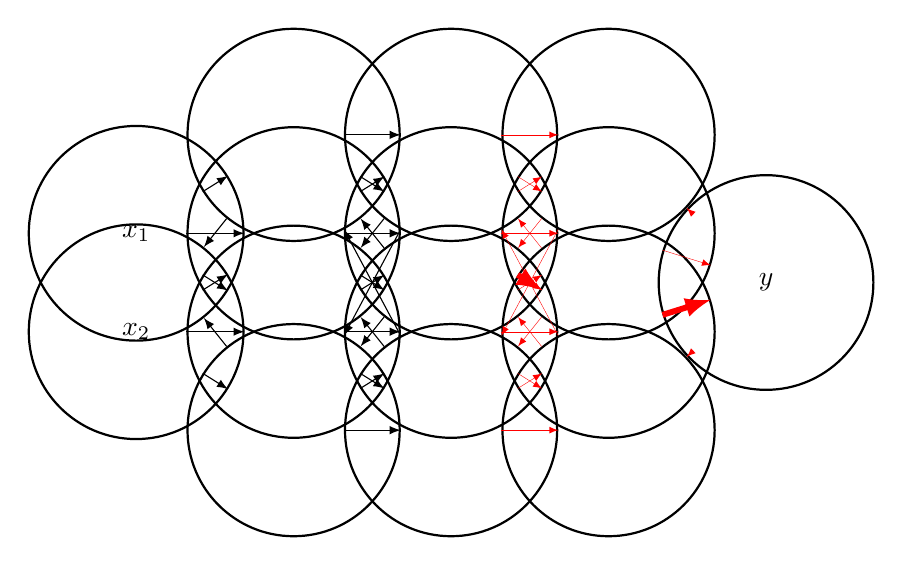
\begin{tikzpicture}
        	\tikzstyle{place}=[circle, draw=black, minimum size = 8mm]
        	% Input
        	\foreach \x in {1,...,2}
        		\draw node at (0, -1.25-\x*1.25) [place] (first_\x) {$x_\x$};
        	% Hidden 1
         	\foreach \x in {1,...,4}
         		\node at (2, -\x*1.25) [place] (second_\x){};%{$n_{1,\x}$};
        	% Hidden 2
        	\foreach \x in {1,...,4}
        		\node at (4, -\x*1.25) [place] (third_\x){};%{$n_{2,\x}$};
        	% Hidden 3
         	\foreach \x in {1,...,4}
         		\node at (6, -\x*1.25) [place] (fourth_\x){};%{$n_{3,\x}$};
        	% Output
        	\foreach \x in {1,...,1}
            		\node at (8, -\x*3.125) [place] (fifth_\x){$y$};
        	%---------------------%
        	% Input -> Hidden 1
        	\foreach \i in {1,...,2}
        		\foreach \j in {1,...,4}
        			\draw [latex-] (first_\i) to (second_\j);
        	% Hidden 1 -> Hidden 2
        	\foreach \i in {1,...,4}
        		\foreach \j in {1,...,4}
        			\draw [latex-] (second_\i) to (third_\j);
        	% Hidden 1 -> Hidden 3
        	\foreach \i in {1,...,4}
        		\foreach \j in {1,...,4}
        			\draw[red, line width=0.05mm] [latex-] (third_\i) to (fourth_\j);
        	\draw[red, line width=0.75mm] [latex-] (third_2) to (fourth_3);
        	% Hidden 3 -> Output
        	\foreach \i in {1,2,4}
    		\foreach \j in {1,...,1}
        			\draw[red, line width=0.05mm] [latex-] (fourth_\i) to (fifth_\j);
        	\draw[red, line width=0.75mm] [latex-] (fourth_3) to (fifth_1);
            %---------------------%
        \end{tikzpicture}
        \caption{Segundo pase}
        \label{fig:back_2}
    \end{figure}
    
    \begin{figure}[h!]
        \centering
        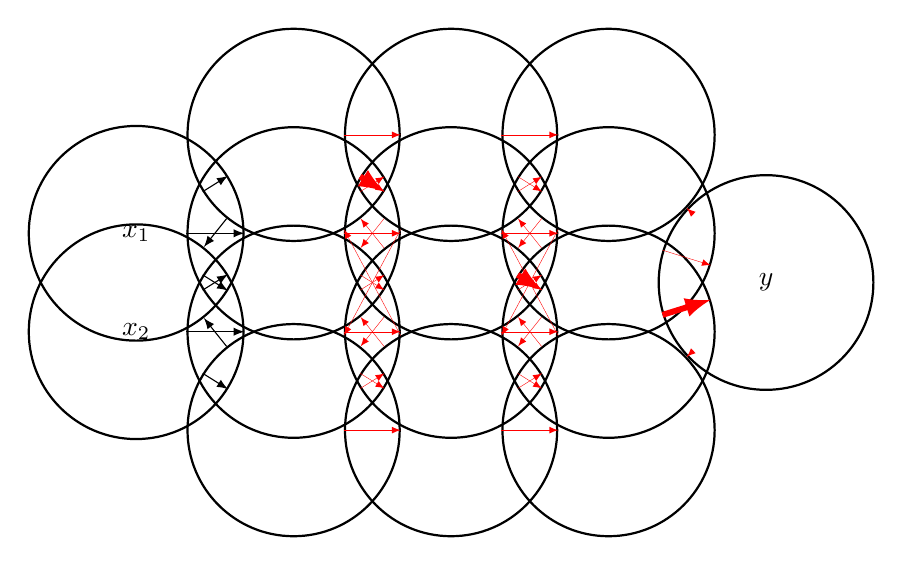
\begin{tikzpicture}
        	\tikzstyle{place}=[circle, draw=black, minimum size = 8mm]
        	% Input
        	\foreach \x in {1,...,2}
        		\draw node at (0, -1.25-\x*1.25) [place] (first_\x) {$x_\x$};
        	% Hidden 1
         	\foreach \x in {1,...,4}
         		\node at (2, -\x*1.25) [place] (second_\x){};%{$n_{1,\x}$};
        	% Hidden 2
        	\foreach \x in {1,...,4}
        		\node at (4, -\x*1.25) [place] (third_\x){};%{$n_{2,\x}$};
        	% Hidden 3
         	\foreach \x in {1,...,4}
         		\node at (6, -\x*1.25) [place] (fourth_\x){};%{$n_{3,\x}$};
        	% Output
        	\foreach \x in {1,...,1}
            		\node at (8, -\x*3.125) [place] (fifth_\x){$y$};
        	%---------------------%
        	% Input -> Hidden 1
        	\foreach \i in {1,...,2}
        		\foreach \j in {1,...,4}
        			\draw [latex-] (first_\i) to (second_\j);
        	% Hidden 1 -> Hidden 2
        	\foreach \i in {1,...,4}
        		\foreach \j in {1,...,4}
        			\draw[red, line width=0.05mm] [latex-] (second_\i) to (third_\j);
        	\draw[red, line width=0.75mm] [latex-] (second_1) to (third_2);
        	% Hidden 1 -> Hidden 3
        	\foreach \i in {1,...,4}
        		\foreach \j in {1,...,4}
        			\draw[red, line width=0.05mm] [latex-] (third_\i) to (fourth_\j);
        	\draw[red, line width=0.75mm] [latex-] (third_2) to (fourth_3);
        	% Hidden 3 -> Output
        	\foreach \i in {1,2,4}
    		\foreach \j in {1,...,1}
        			\draw[red, line width=0.05mm] [latex-] (fourth_\i) to (fifth_\j);
        	\draw[red, line width=0.75mm] [latex-] (fourth_3) to (fifth_1);
            %---------------------%
        \end{tikzpicture}
        \caption{Tercer pase}
        \label{fig:back_3}
    \end{figure}

    \begin{figure}[h!]
        \centering
        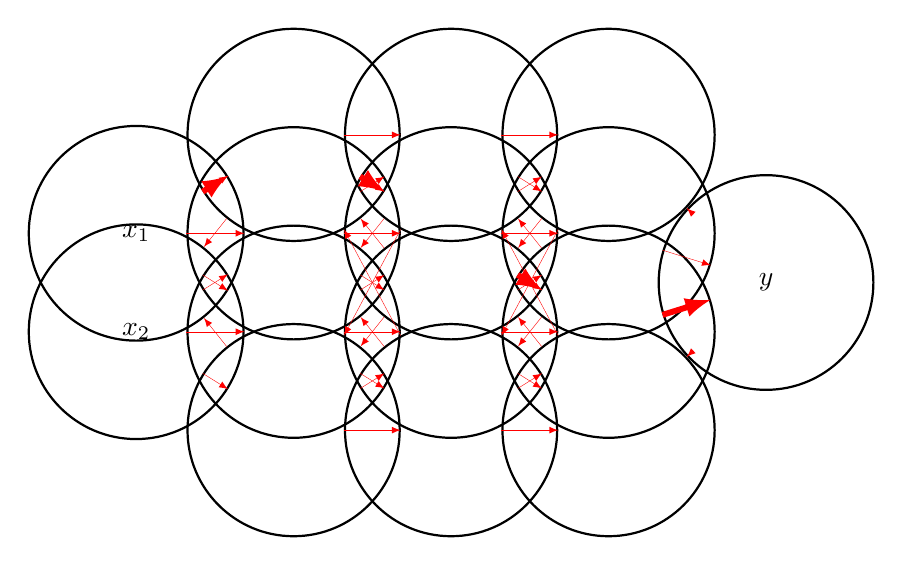
\begin{tikzpicture}
        	\tikzstyle{place}=[circle, draw=black, minimum size = 8mm]
        	% Input
        	\foreach \x in {1,...,2}
        		\draw node at (0, -1.25-\x*1.25) [place] (first_\x) {$x_\x$};
        	% Hidden 1
         	\foreach \x in {1,...,4}
         		\node at (2, -\x*1.25) [place] (second_\x){};%{$n_{1,\x}$};
        	% Hidden 2
        	\foreach \x in {1,...,4}
        		\node at (4, -\x*1.25) [place] (third_\x){};%{$n_{2,\x}$};
        	% Hidden 3
         	\foreach \x in {1,...,4}
         		\node at (6, -\x*1.25) [place] (fourth_\x){};%{$n_{3,\x}$};
        	% Output
        	\foreach \x in {1,...,1}
            		\node at (8, -\x*3.125) [place] (fifth_\x){$y$};
        	%---------------------%
        	% Input -> Hidden 1
        	\foreach \i in {1,...,2}
        		\foreach \j in {1,...,4}
        			\draw[red, line width=0.05mm] [latex-] (first_\i) to (second_\j);
        	\draw[red, line width=0.75mm] [latex-] (first_1) to (second_1);
        	% Hidden 1 -> Hidden 2
        	\foreach \i in {1,...,4}
        		\foreach \j in {1,...,4}
        			\draw[red, line width=0.05mm] [latex-] (second_\i) to (third_\j);
        	\draw[red, line width=0.75mm] [latex-] (second_1) to (third_2);
        	% Hidden 1 -> Hidden 3
        	\foreach \i in {1,...,4}
        		\foreach \j in {1,...,4}
        			\draw[red, line width=0.05mm] [latex-] (third_\i) to (fourth_\j);
        	\draw[red, line width=0.75mm] [latex-] (third_2) to (fourth_3);
        	% Hidden 3 -> Output
        	\foreach \i in {1,2,4}
    		\foreach \j in {1,...,1}
        			\draw[red, line width=0.05mm] [latex-] (fourth_\i) to (fifth_\j);
        	\draw[red, line width=0.75mm] [latex-] (fourth_3) to (fifth_1);
            %---------------------%
        \end{tikzpicture}
        \caption{Cuarto pase}
        \label{fig:back_4}
    \end{figure}
    
\end{itemize}

\clearpage

% -- -- %


\section{IA aplicado a la monitorización estructural}

TODOS los sectores menos aeronáutica - entre 5 y 10 pags 

Poner un estado actuar de como se esta aplicando la IA a la monitorización estructuras en general

\clearpage

% -- -- %


\section{IA aplicada a la monitorización de estructuras aeronáuticas}

INESASSE (5 pags VER TFM Jaime García SOLO INTRODUCIR)

Dar una vuelta al apartado anterior centrándolo sobre todo en estructuras aeronáuticas. Si se puede, poner ejemplos de estructuras de material compuesto e inferir en la complejidad que dan frente a las metálicas por su direccionalidad de propiedades.



\section{RNN LSTM}

Esplicación completa y detallada

\clearpage

%  --  --  %
